\documentclass[10pt]{article}
\usepackage{fullpage}
\usepackage{graphicx}
\usepackage{booktabs}
\title{Supplementary data and evaluation results for ``idock: Improving Docking Speed over AutoDock Vina and istar: Software-as-a-Service Platform for idock"}
\pagestyle{empty}
\begin{document}
\maketitle
\thispagestyle{empty}

\pagebreak
\begin{table}
\centering
\begin{tabular*}
{\linewidth}
{@{\extracolsep{\fill}}crrrr}
\toprule
& \multicolumn{2}{c}{PDBbind v2011} & \multicolumn{2}{c}{CSAR NRC HiQ}\\
Condition & idock & Vina & idock & Vina\\
\midrule
RMSD1 = RMSDm           & 47\% & 54\% & 57\% & 71\%\\
RMSD2 = RMSDm           & 16\% & 14\% & 17\% & 13\%\\
RMSD3 = RMSDm           &  8\% &  8\% &  7\% &  4\%\\
RMSD4 = RMSDm           &  6\% &  5\% &  5\% &  3\%\\
RMSD5 = RMSDm           &  5\% &  5\% &  4\% &  1\%\\
RMSD6 = RMSDm           &  5\% &  4\% &  3\% &  3\%\\
RMSD7 = RMSDm           &  5\% &  4\% &  1\% &  2\%\\
RMSD8 = RMSDm           &  4\% &  3\% &  3\% &  2\%\\
RMSD9 = RMSDm           &  4\% &  3\% &  3\% &  2\%\\
\noalign{\smallskip}
RMSD1 \textless\ 0.5 \AA & 11\% & 12\% & 21\% & 21\%\\
RMSD1 \textless\ 1.0 \AA & 29\% & 31\% & 40\% & 47\%\\
RMSD1 \textless\ 1.5 \AA & 45\% & 47\% & 61\% & 67\%\\
RMSD1 \textless\ 2.0 \AA & 53\% & 56\% & 68\% & 73\%\\
\noalign{\smallskip}
RMSDm \textless\ 0.5 \AA & 14\% & 15\% & 24\% & 26\%\\
RMSDm \textless\ 1.0 \AA & 39\% & 40\% & 54\% & 55\%\\
RMSDm \textless\ 1.5 \AA & 64\% & 65\% & 78\% & 84\%\\
RMSDm \textless\ 2.0 \AA & 74\% & 78\% & 86\% & 92\%\\
\bottomrule
\end{tabular*}
\caption{Redocking benchmark results: redocking success rates of idock and AutoDock Vina on PDBbind v2011 and CSAR NRC HiQ Set 24Sept2010 under various conditions regarding the RMSD (Root Mean Square Deviation) values between the crystal and docked conformations. Arguments to both programs were left as default. Both programs output 9 conformations per ligand by default. RMSD1 refers to the RMSD value between the crystal conformation and the first docked conformation with the highest predicted binding affinity, while RMSDm refers to the RMSD value between the crystal conformation and the closest docked conformation with the lowest RMSD value. The condition RMSD1 = RMSDm therefore tests for how many percent the docked conformation with the highest predicted binding affinity actually turns out to be the closest one among the 9 predicted conformations. It can be seen that the success rates of idock were comparable to, albeit slightly lower than, AutoDock Vina. Using a RMSD value of 2.0 \AA, a publicly accepted positive control for correct bound structure prediction, both programs managed to predict a conformation close enough to the crystal conformation as the first conformation for over half of the cases on both datasets.}
\label{idock:SuccessRate}
\end{table}

\pagebreak
\begin{table}
\centering
\begin{tabular*}
{\linewidth}
{@{\extracolsep{\fill}}crrrrrr}
\toprule
& \multicolumn{2}{c}{200-300g/mol} & \multicolumn{2}{c}{300-400g/mol} & \multicolumn{2}{c}{400-500g/mol}\\
& CPU & Elapsed & CPU & Elapsed & CPU & Elapsed\\
\midrule
\multicolumn{7}{l}{\textbf{1HCL} human cyclin-dependent kinase 2}\\
Vina  & 12.57 &  3.33 & 22.55 &  5.91 & 51.62 & 13.41\\
idock &  0.63 &  0.16 &  0.92 &  0.24 &  1.38 &  0.36\\
Ratio & 20.06 & 20.25 & 24.41 & 24.39 & 37.51 & 36.81\\
\multicolumn{7}{l}{\textbf{1J1B} human tau protein kinase I}\\
Vina  &  9.07 &  2.47 & 14.69 &  3.92 & 32.28 &  8.49\\
idock &  0.78 &  0.21 &  1.25 &  0.33 &  2.35 &  0.62\\
Ratio & 11.55 & 11.92 & 11.73 & 11.87 & 13.73 & 13.73\\
\multicolumn{7}{l}{\textbf{1LI4} human S-adenosylhomocysteine hydrolase}\\
Vina  & 11.82 &  3.30 & 19.08 &  5.22 & 39.41 & 10.64\\
idock &  0.89 &  0.23 &  1.55 &  0.40 &  3.15 &  0.82\\
Ratio & 13.24 & 14.14 & 12.33 & 12.95 & 12.50 & 12.98\\
\multicolumn{7}{l}{\textbf{1V9U} human rhinovirus 2 coat protein VP1}\\
Vina  &  9.80 &  2.95 & 15.55 &  4.62 & 29.75 &  8.49\\
idock &  0.97 &  0.25 &  1.64 &  0.42 &  3.42 &  0.89\\
Ratio & 10.11 & 11.74 &  9.49 & 10.91 &  8.69 &  9.56\\
\multicolumn{7}{l}{\textbf{2IQH} influenza A virus nucleoprotein NP}\\
Vina  &  9.51 &  2.66 & 15.03 &  4.08 & 29.64 &  7.83\\
idock &  0.92 &  0.24 &  1.59 &  0.41 &  3.41 &  0.88\\
Ratio & 10.35 & 11.18 &  9.43 &  9.93 &  8.69 &  8.93\\
\multicolumn{7}{l}{\textbf{2XSK} Escherichia coli curli protein CsgC - SeCys}\\
Vina  & 10.44 &  2.71 & 17.89 &  4.61 & 40.58 & 10.41\\
idock &  0.71 &  0.19 &  1.16 &  0.30 &  2.16 &  0.56\\
Ratio & 14.68 & 14.64 & 15.47 & 15.38 & 18.83 & 18.57\\
\multicolumn{7}{l}{\textbf{2ZD1} HIV-1 reverse transcriptase}\\
Vina  &  9.78 &  2.70 & 17.67 &  4.76 & 42.03 & 11.33\\
idock &  0.97 &  0.25 &  1.52 &  0.39 &  2.60 &  0.69\\
Ratio & 10.05 & 10.73 & 11.61 & 12.07 & 16.14 & 16.54\\
\multicolumn{7}{l}{\textbf{2ZNL} influenza virus RNA polymerase subunit PA}\\
Vina  &  9.49 &  2.60 & 15.04 &  4.01 & 29.97 &  7.82\\
idock &  0.89 &  0.23 &  1.56 &  0.40 &  3.41 &  0.87\\
Ratio & 10.70 & 11.37 &  9.65 & 10.06 &  8.78 &  8.98\\
\multicolumn{7}{l}{\textbf{3BGS} human purine nucleoside phosphorylase}\\
Vina  &  9.59 &  2.57 & 16.50 &  4.37 & 38.42 & 10.14\\
idock &  0.95 &  0.25 &  1.55 &  0.40 &  2.81 &  0.74\\
Ratio & 10.09 & 10.45 & 10.65 & 10.89 & 13.65 & 13.75\\
\multicolumn{7}{l}{\textbf{3H0W} human S-adenosylmethionine decarboxylase}\\
Vina  &  9.85 &  2.64 & 17.67 &  4.70 & 41.69 & 11.04\\
idock &  0.88 &  0.23 &  1.35 &  0.35 &  2.20 &  0.58\\
Ratio & 11.17 & 11.50 & 13.07 & 13.28 & 18.99 & 19.11\\
\multicolumn{7}{l}{\textbf{3IAR} human adenosine deaminase}\\
Vina  & 11.25 &  3.03 & 20.21 &  5.39 & 46.93 & 12.53\\
idock &  0.80 &  0.21 &  1.21 &  0.32 &  2.01 &  0.53\\
Ratio & 14.10 & 14.44 & 16.68 & 16.90 & 23.34 & 23.59\\
\multicolumn{7}{l}{\textbf{3KFN} HIV protease}\\
Vina  & 10.53 &  2.80 & 18.37 &  4.83 & 42.43 & 11.03\\
idock &  0.77 &  0.20 &  1.20 &  0.32 &  2.09 &  0.55\\
Ratio & 13.69 & 13.85 & 15.29 & 15.32 & 20.32 & 20.12\\
\multicolumn{7}{l}{\textbf{Average across the above 12 receptors}}\\
Vina  & 10.31 &  2.81 & 17.52 &  4.70 & 38.73 & 10.26\\
idock &  0.85 &  0.22 &  1.38 &  0.36 &  2.58 &  0.67\\
Ratio & 12.48 & 13.02 & 13.32 & 13.66 & 16.76 & 16.89\\
\bottomrule
\end{tabular*}
\caption{Virtual screening benchmark results: CPU time and elapsed time in hours of docking 3000 clean ligands of 3 molecular weight sets against 12 diverse receptors by AutoDock Vina and idock. Typically idock outperformed Vina by at least 8.69 times and at most 37.51 times in terms of docking speed.}
\label{idock:ExecutionTime}
\end{table}

\pagebreak
\begin{figure}
\centering
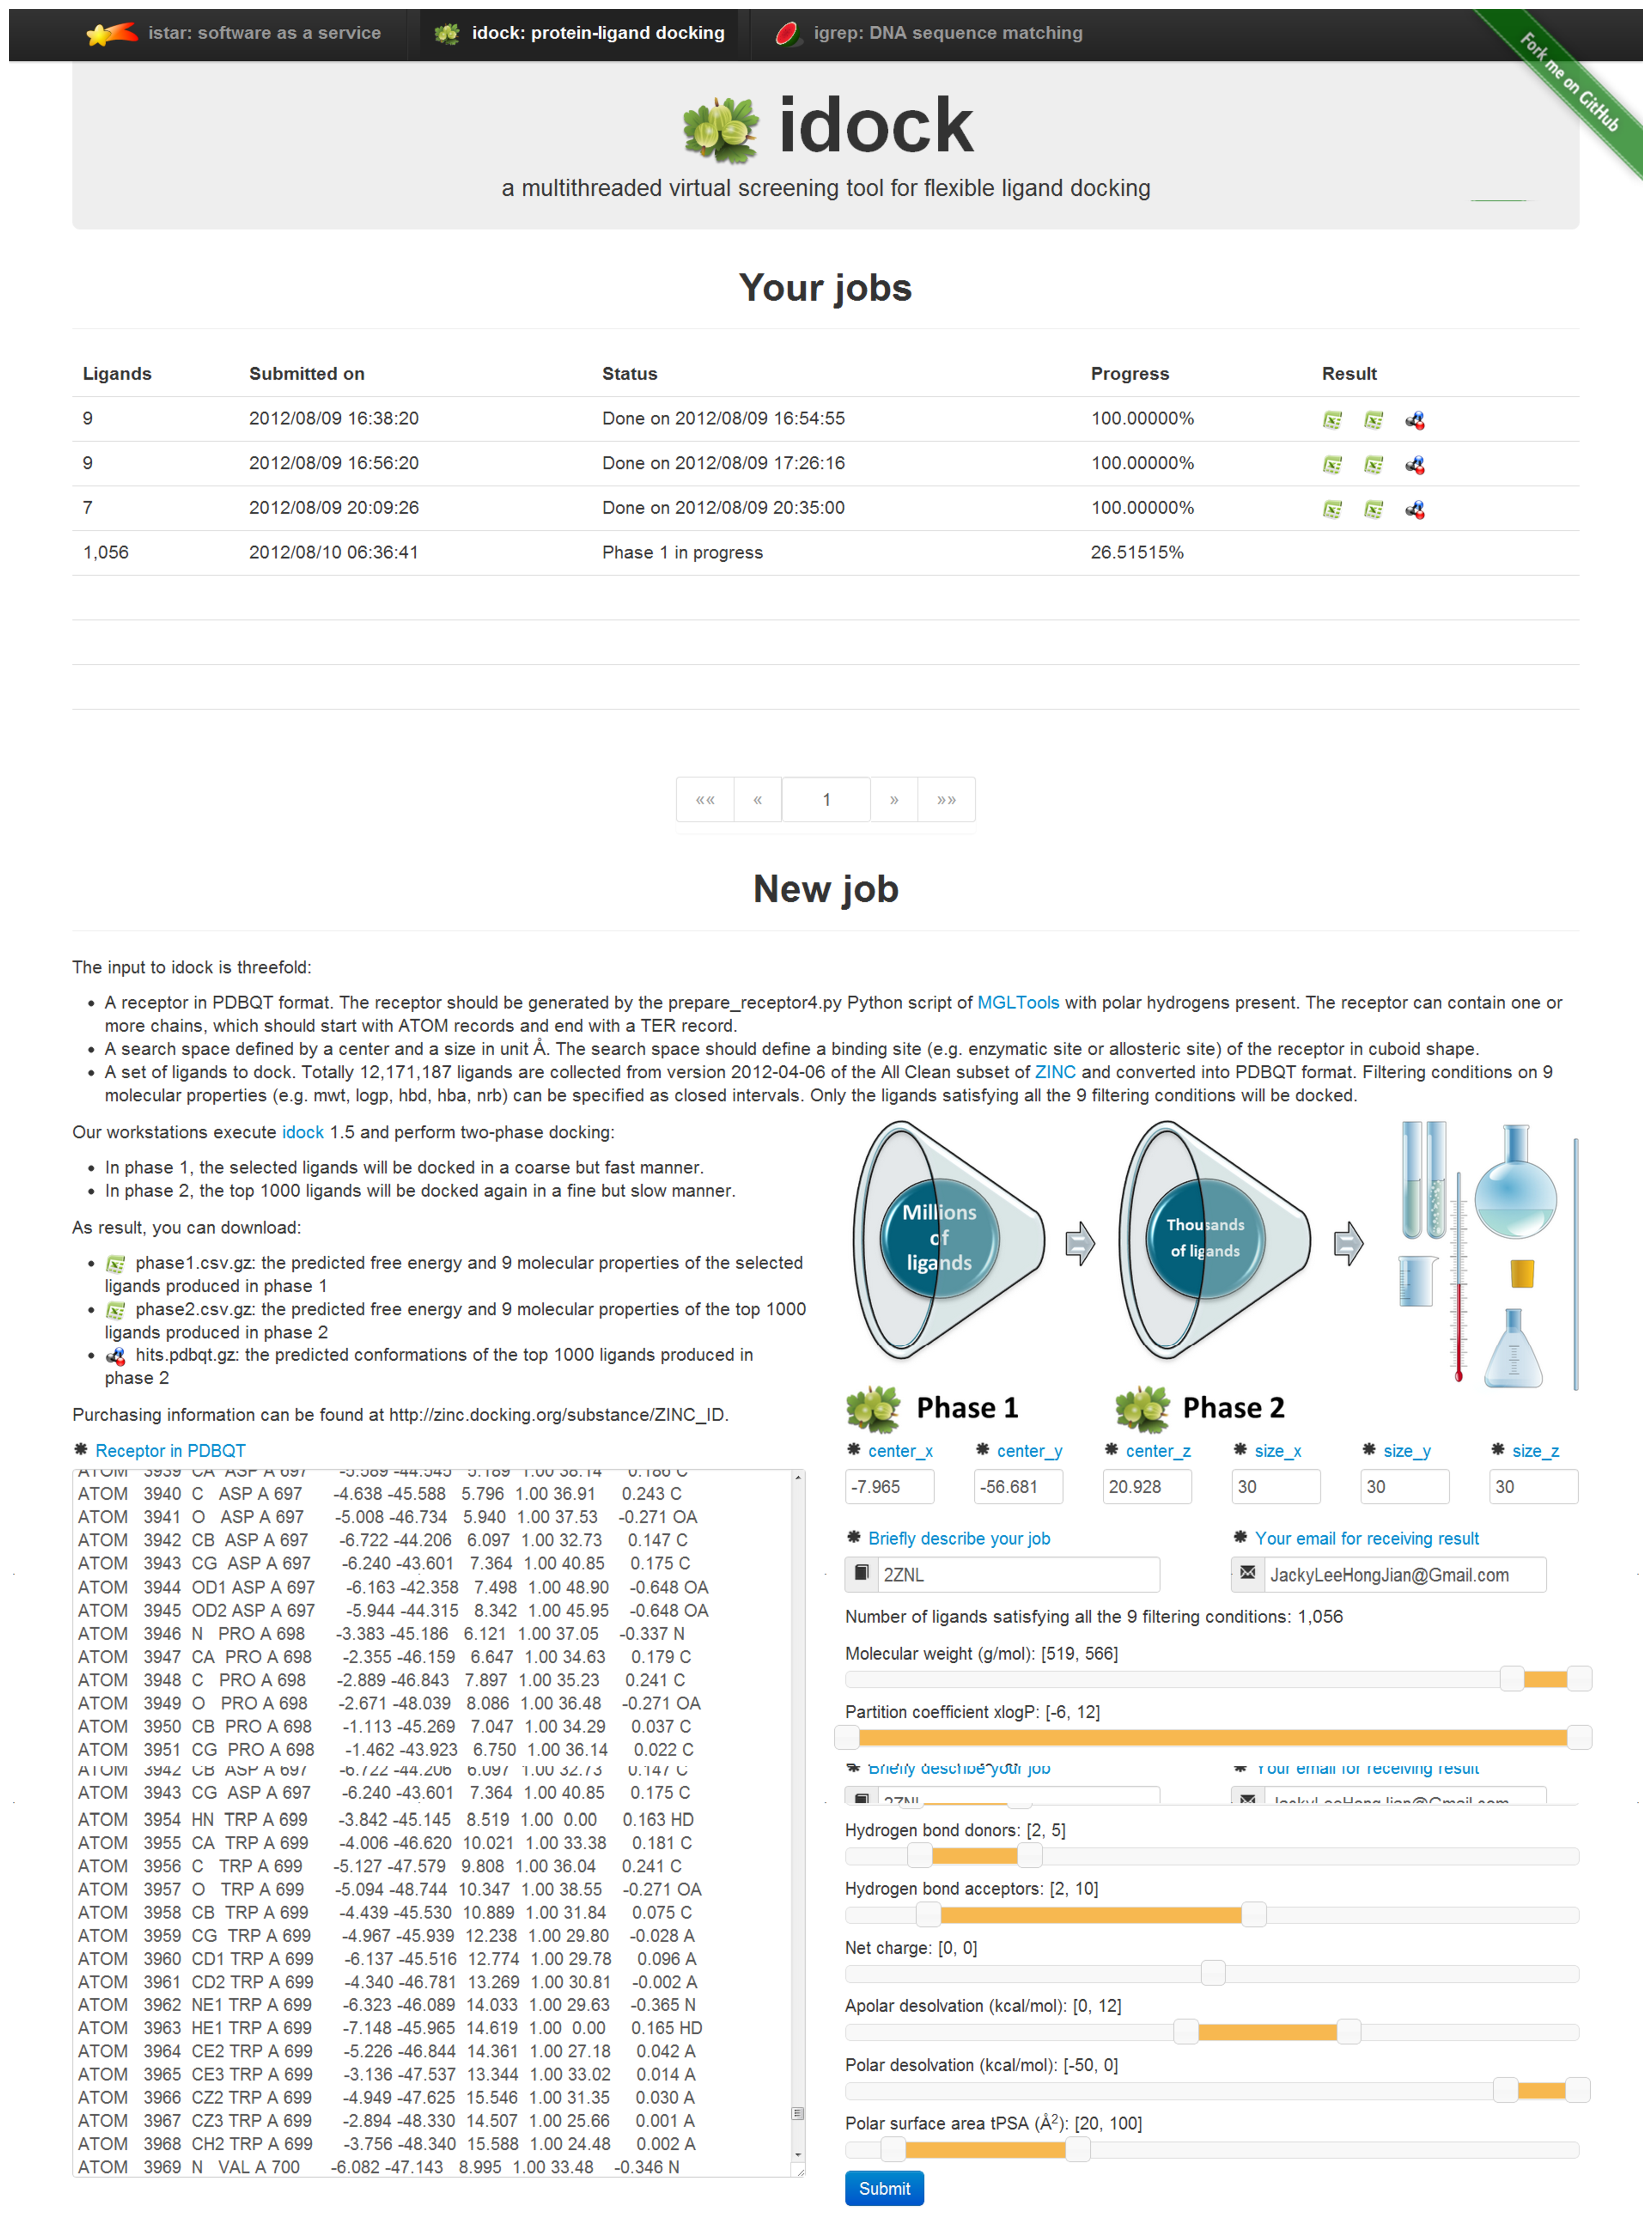
\includegraphics[width=0.8\linewidth]{idock.eps}
\caption{The online version of idock is hosted by istar and available at http://istar.cse.cuhk.edu.hk/idock. We have seamlessly combined both the Twitter Bootstrap and the HTML5 Boilerplate into a HTML5- and CSS3-powered web site, which has been successfully checked as HTML5 by the W3C Markup Validator v1.3. We have adopted the jQuery library to simplify HTML document traversing, event handling, animating, and Ajax interactions, and the jQuery UI library to provide themeable widgets. We have tested our web site with Chrome 19+, Firefox 12+, Internet Explorer 9+, Safari 5+ and Opera 12+. Our idock web page supports filtering and previewing ligands to dock, as well as monitoring job progress in real time, two very useful and unique features only available at istar. A new job consists of compulsory fields as well as optional fields. Compulsory fields include a receptor in PDBQT format, a search space defined by a cubic box, a short description of the job, and an email to receive completion notification. Optional fields include filtering conditions of ligands on 9 molecular properties, e.g. molecular weight and partition coefficient xlogP. We have set up default values for optional fields, and only the ligands satisfying all the 9 filtering conditions will be docked. We have also recorded a video tutorial for newbies to get started easily.}
\label{istar:idock}
\end{figure}

\pagebreak
\begin{figure}
\centering
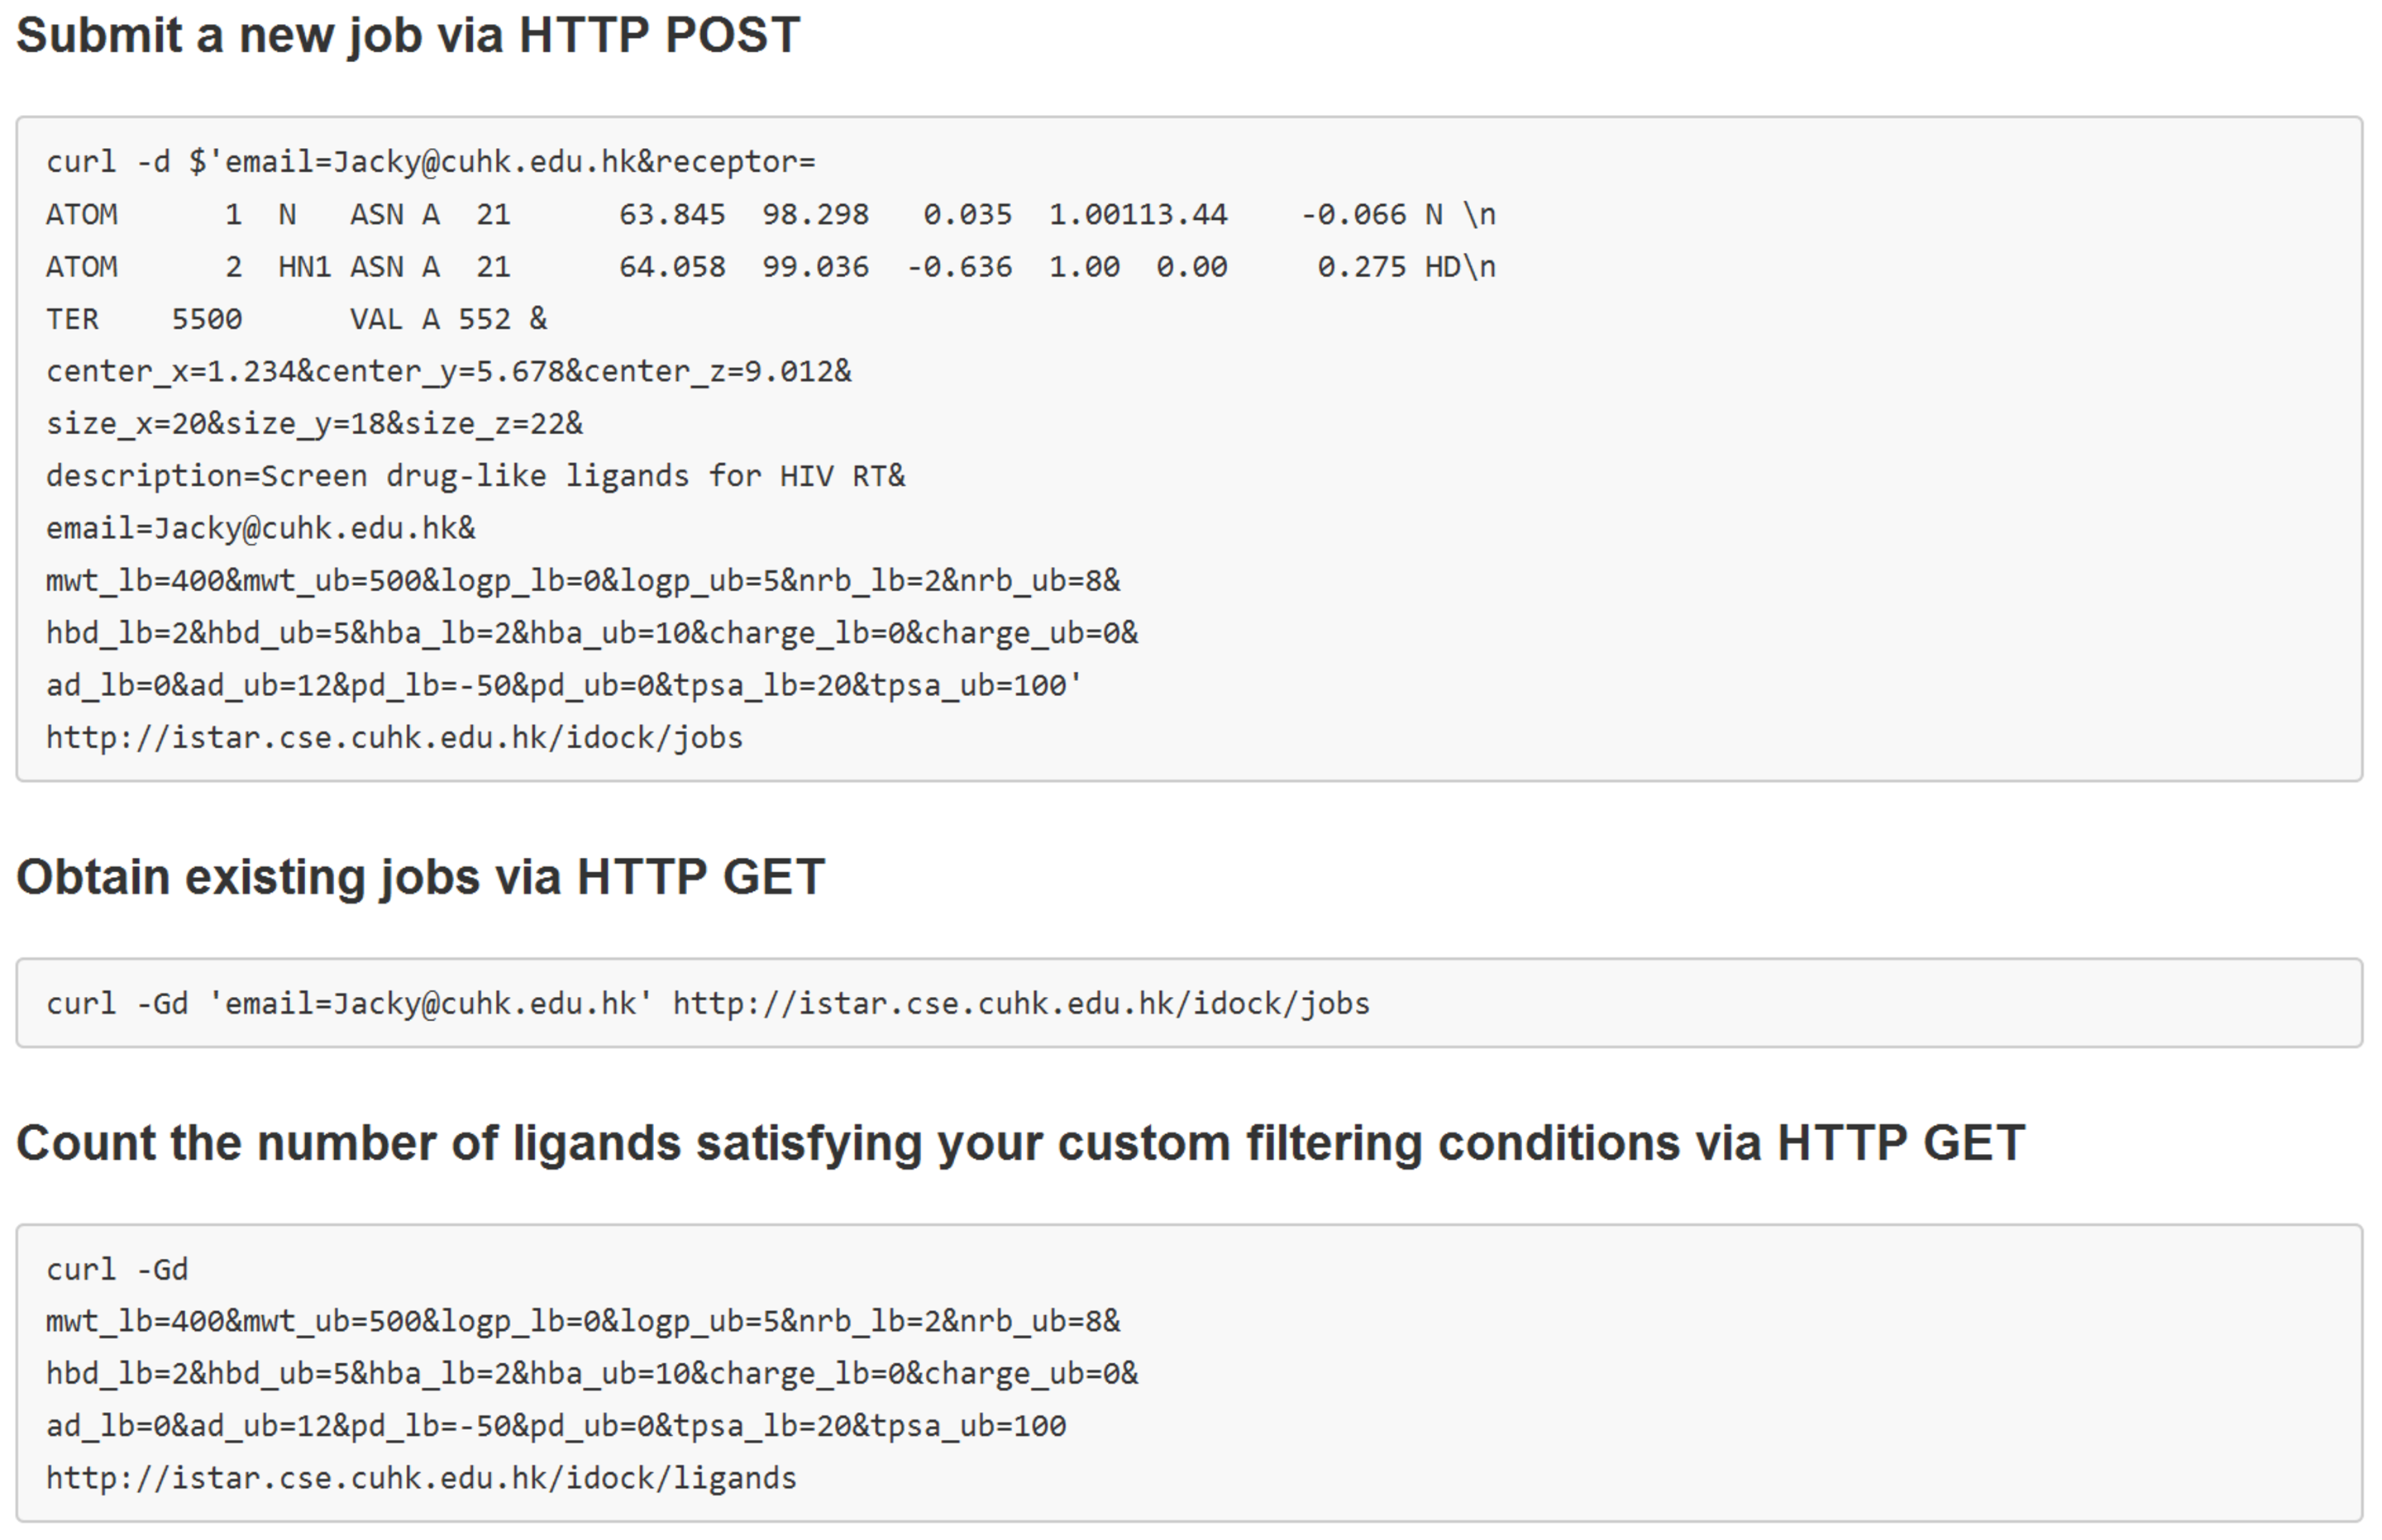
\includegraphics[width=\linewidth]{idock-rest.eps}
\caption{RESTful API of idock. We have exposed job submission, job query, and ligand counting as RESTful API for others to program against. Under Unix-like operating systems, one can use the ``curl" utility to trigger our RESTful API. Refer to the idock web site for more detail.}
\label{istar:idock-rest}
\end{figure}

\end{document}
